\documentclass[]{beamer}

\mode<presentation> {
	%\usetheme{default}
	%\usetheme{AnnArbor}
	%\usetheme{Antibes}
	%\usetheme{Bergen}
	%\usetheme{Berkeley}
	%\usetheme{Berlin}
	%\usetheme{Boadilla}
	%\usetheme{CambridgeUS}
	%\usetheme{Copenhagen}
	%\usetheme{Darmstadt}
	%\usetheme{Dresden}
	%\usetheme{Frankfurt}
	%\usetheme{Goettingen}
	%\usetheme{Hannover}
	%\usetheme{Ilmenau}
	%\usetheme{JuanLesPins}
	%\usetheme{Luebeck}
	\usetheme{Madrid}
	%\usetheme{Malmoe}
	%\usetheme{Marburg}
	%\usetheme{Montpellier}
	%\usetheme{PaloAlto}
	%\usetheme{Pittsburgh}
	%\usetheme{Rochester}
	%\usetheme{Singapore}
	%\usetheme{Szeged}
	%\usetheme{Warsaw}

	%\usecolortheme{albatross}
	%\usecolortheme{beetle}
	%\usecolortheme{crane}
	%\usecolortheme{dolphin}
	%\usecolortheme{dove}
	%\usecolortheme{fly}
	%\usecolortheme{lily}
	%\usecolortheme{orchid}
	%\usecolortheme{rose}
	%\usecolortheme{seagull}
	%\usecolortheme{seahorse}
	%\usecolortheme{whale}
	%\usecolortheme{wolverine}
}

\usepackage[russian]{babel}
\usepackage[utf8]{inputenc}
%\usepackage[T2A]{fontenc}
%\usepackage[T1]{fontenc}
%\usepackage{tgtermes}
\usepackage{verbatim}
%\usepackage{minted}

%\usepackage{citehack} 
%\usepackage{tikz}
%\usetikzlibrary{patterns}

%\usepackage{amsmath}
%\usepackage{amsfonts}
%\usepackage{pgfplots}
\usepackage{hyperref}
\usepackage{graphics, graphicx}

%\usepackage{color}
%\usepackage{enumerate}
%\usepackage{booktabs}
%\usepackage{mathtools}
%\usepackage{algorithm}
%\usepackage[noend]{algpseudocode}
%\usepackage{latexsym}
%\usepackage{mdframed}
%\usepackage{minted}
%\usemintedstyle{default}
%\usepackage[noend]{algorithmic}

\title[Git]{\bfseries Система контроля версий git. Методика git-flow}
\author[Cолоткий~М.]{Солоткий Михаил}
\institute[ВМК МГУ]{МГУ имени М. В. Ломоносова, факультет ВМК, кафедра ММП}
\date{27 марта 2019 года}

\begin{document}

%\medskip

\begin{frame}
	\titlepage
\end{frame}

\begin{frame} \frametitle{Что такое система контроля версий}
	\begin{itemize}
		\item Система контроля версий (СКВ) — это система, регистрирующая изменения в одном или нескольких файлах с тем, чтобы в дальнейшем была возможность вернуться к определённым старым версиям этих файлов. \newline \par

		\item Кому может пригодиться:
		\begin{itemize}
		    \item Разработчикам;
		    \item Аналитикам;
		    \item Исследователям.
		\end{itemize}
	\end{itemize}
\end{frame}

\begin{frame} \frametitle{Зачем нужны СКВ}
\begin{itemize}
		\item Зачем нужна:
		\begin{itemize}
		    \item Если что-то будет испорчено, это можно легко восстановить;
             \item Хранит время и автора изменения;
		    \item Удобно хранить неудачные версии;
		    \item Автоматизация совместной работы над проектом;
		    \begin{itemize}
		        \item Каждый ответственен за свою некоторую часть проекта и вносит изменения по ней;
		        \item Можно совместно писать научную статью.
		    \end{itemize}
		\end{itemize}
\end{itemize}
\end{frame}

\begin{frame} \frametitle{Самое важное, что нужно знать о git}
	\begin{itemize}
		\item Как инициировать контроль версий;
		\item Как делать коммиты;
		\item Как переключиться на другую версию;
		\item Как создавать, переключаться, удалять и сливать ветки;
		\item Как работать с удалённым сервером;
		\item Как разрешать конфликты
		\item[~]
	\end{itemize}
	Книга по пользованию git: \newline
	\url{https://git-scm.com/book/ru/v1/}
\end{frame}

\begin{frame} \frametitle{Преимущества Git}
	\begin{itemize}
		\item Быстрое переключение между версиями (в отличие от CVS, Subversion, Perforce, Bazaar); \newline \par
		\item Git - распределённая система (в отличие от CVS, Subversion и Perforce); \newline \par
		\item Git следит за безопасностью данных. \newline \par
	\end{itemize}
\end{frame}

\begin{frame} \frametitle{Что такое git-flow}
	\begin{itemize}
		\item git-flow - набор рекомендаций разработчикам, базирующийся на работе с различными ветками при приследовании различных целей; \newline \par
		\item master - ветка, хранящая стабильные версии кода;
		\item develop - ветка, в которую разработчики вливают новые протестированные фичи;
		\item feature - ветка для создания новой функциональности или изменения старой, именно в этой ветке разработчики начинают работу над какой-то задачей
		\item release - ветка для релизов, сюда вливается код из ветки develop проводится полное тестирование, назначается тэг версии;
		\item hotfix - для быстрых изменений, вливается потом в master и develop.
	\end{itemize}
\end{frame}

\begin{frame} \frametitle{Пример проекта с git-flow}
\begin{center}
    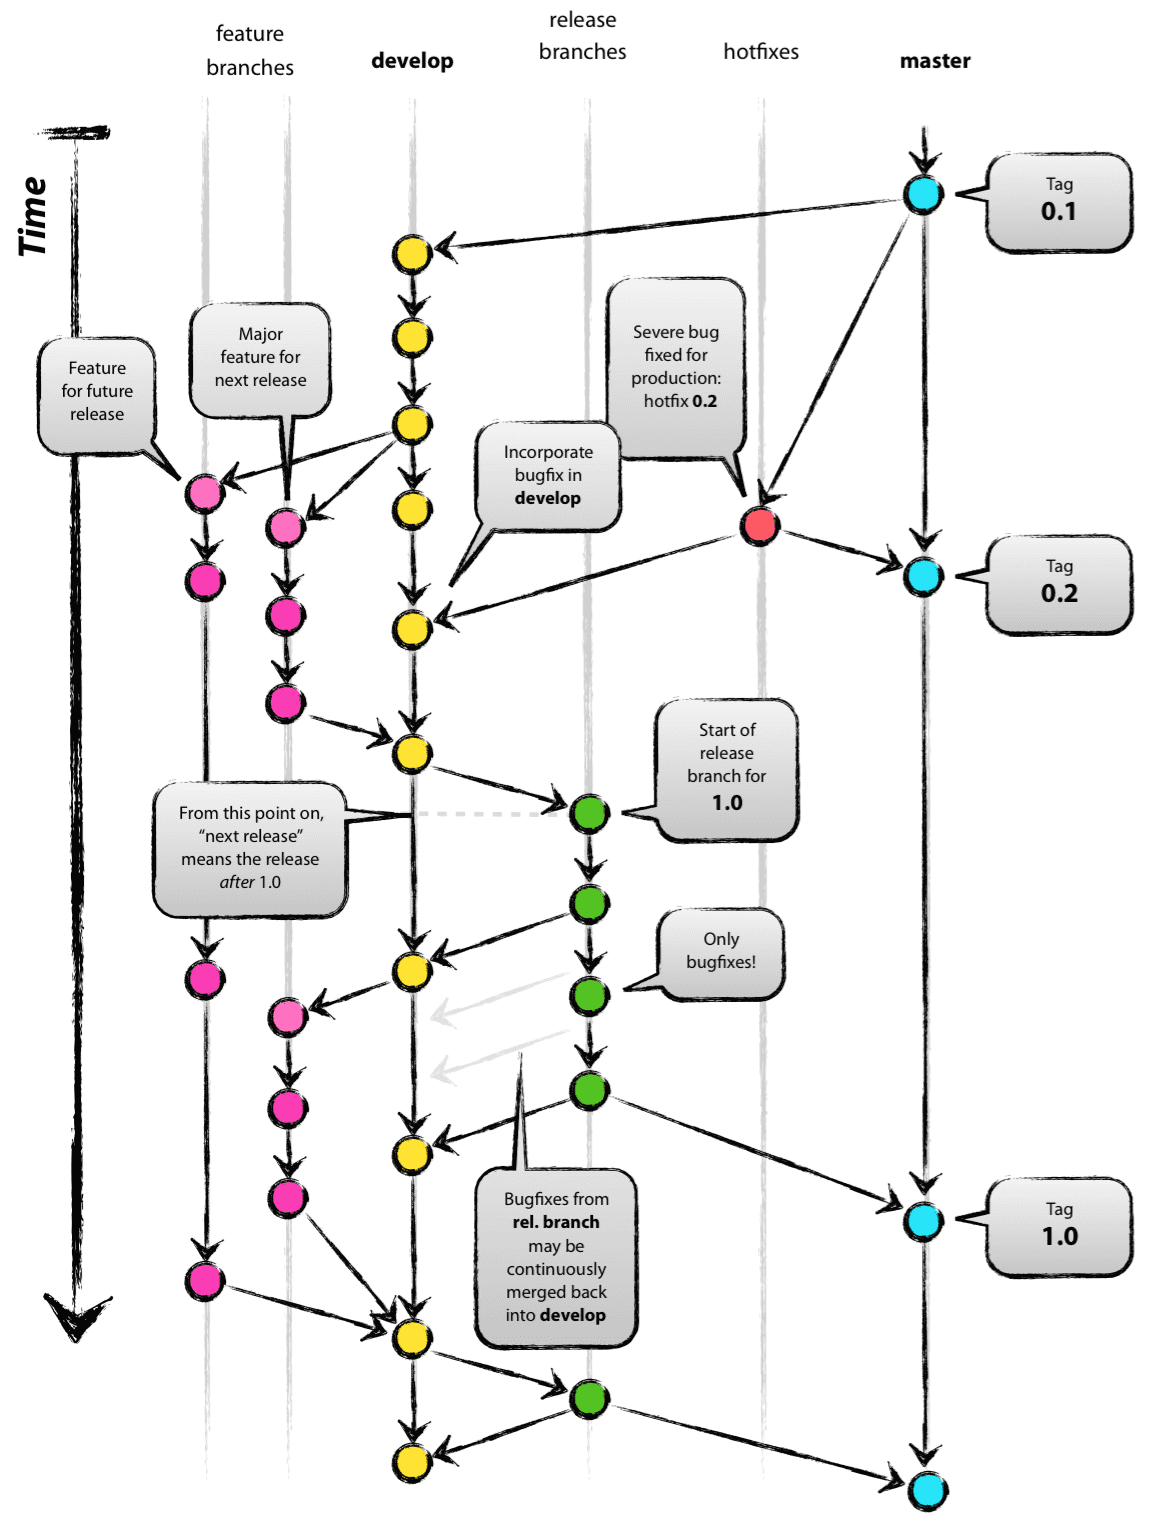
\includegraphics[scale=0.13]{git-model@2x.png}
\end{center}
\end{frame}

\begin{frame} \frametitle{Fork}
\begin{itemize}
    \item Есть приложение, реализующее методологию git-flow, называется Fork
\end{itemize}
\begin{center}
    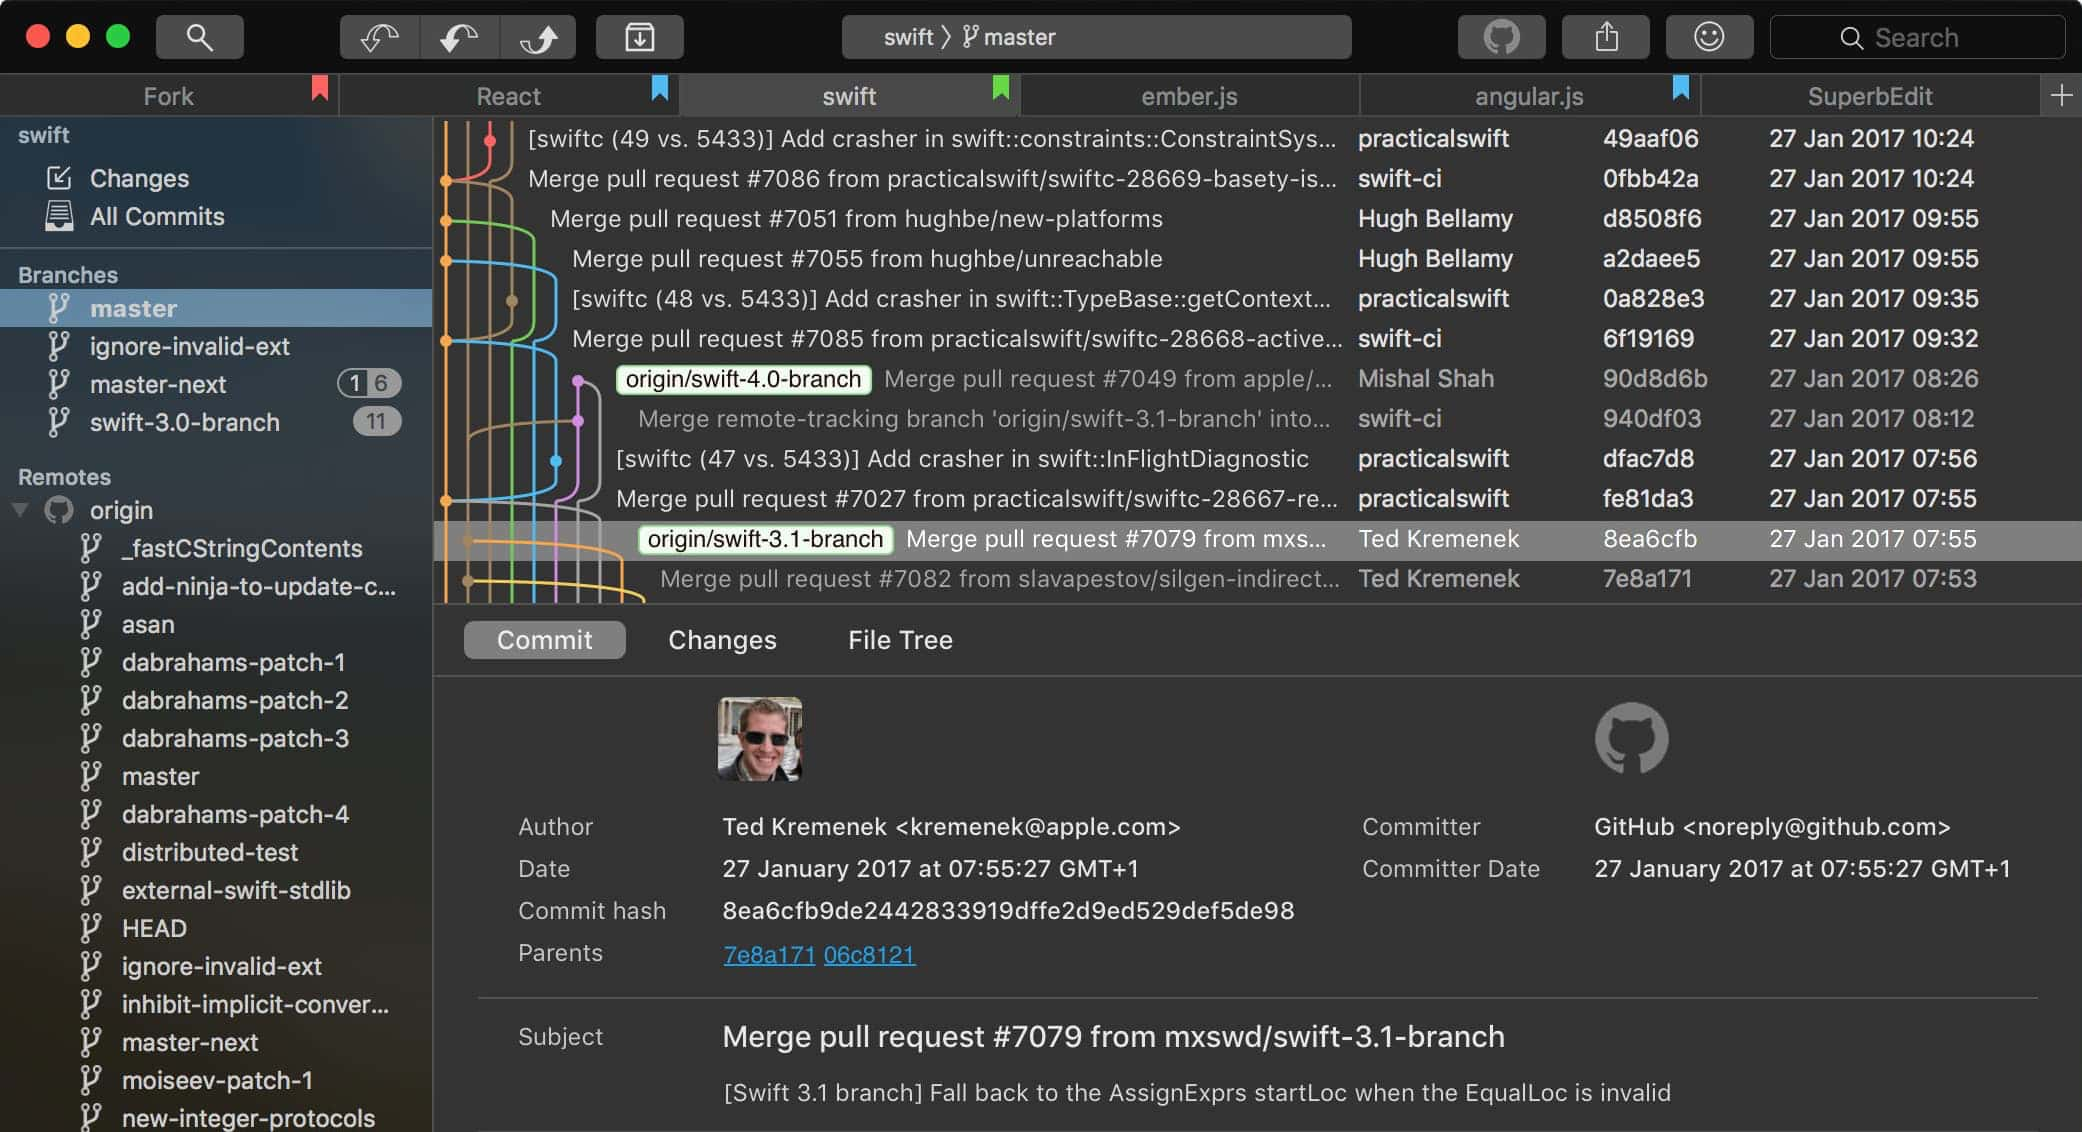
\includegraphics[scale=0.13]{image1.jpg}
\end{center}
\end{frame}

\begin{frame} \frametitle{Выводы}
\begin{itemize}
    \item Git-flow = хорошо, так как позволяет автоматизировать совместную работу, быстро решать hotfix;
    \item Стандартизация работы;
    \item Удобно следовать методологии git-flow, так как она интегрирована в некоторые IDE.
\end{itemize}
\end{frame}

\begin{frame} \frametitle{Где ещё можно почитать о git-flow (clickable)}
\begin{itemize}
    \item \href{https://zellwk.com/blog/git-flow/}{Managing your Git branches with Git Flow (Zellwk's blog)}
    \item \href{https://www.atlassian.com/git/tutorials/comparing-workflows/gitflow-workflow}{Gitflow Workflow with tutolrials}
    \item \href{https://guides.github.com/introduction/flow/}{Understanding the GitHub flow (Github's guide)}
\end{itemize}
\end{frame}

\end{document}